Mars mission launch windows only occur once every 26 months, as showin in \refFig{fig:mars-distance-from-earth}. This section presents the power systems of Mars surface missions planned for the next window.

\begin{figure}[h]
  \captionsetup[subfigure]{justification=centering}
  \centering
  \hypersetup{linkcolor=captionTextColor}
  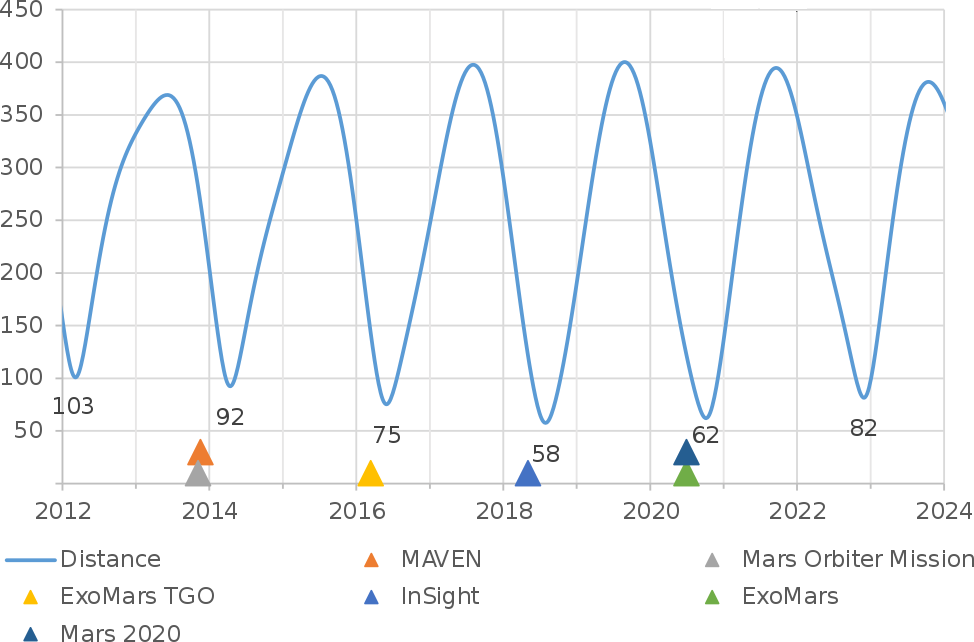
\includegraphics[width=0.5\linewidth]{sections/state-of-the-art/planned-missions/plots/mars-distance-from-earth.png}\\
  \caption[Spacecraft launches and Mars distance from Earth]
          {Spacecraft launches and Mars distance from Earth (Gm). Data source: HORIZONS System, JPL, NASA.}
  \label{fig:mars-distance-from-earth}
\end{figure}

At the time of writing this thesis, two rover missions are set to be launched during the next window: \ac{NASA}'s Mars 2020 rover, shown in \refFig{fig:sub:planned-mission-rover-mars2020}, and the \ac{ESA}/Roscosmos' ExoMars Rosalind Franklin rover, shown in \refFig{fig:sub:planned-mission-rover-exomars}.

\vspace{0.5cm}

\begin{figure}[h]
\captionsetup[subfigure]{justification=centering}
\vspace{-2ex}
	\centering
    %% setup sizes
    \setlength{\graphicsHeight}{50mm}
    %% kill hyper-link highlighting
    \hypersetup{hidelinks=true}%
    %% the figures
	\begin{subfigure}[t]{0.65\textwidth}
        \centering
		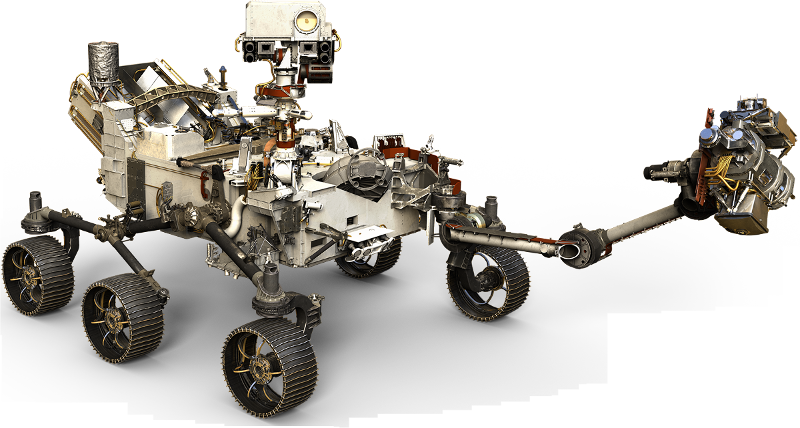
\includegraphics[height=\graphicsHeight]{sections/state-of-the-art/planned-missions/images/rover-mars2020.png}
		\subcaption{Mars 2020}
		\label{fig:sub:planned-mission-rover-mars2020}
	\end{subfigure}\hfill
	\begin{subfigure}[t]{0.35\textwidth}
        \centering
		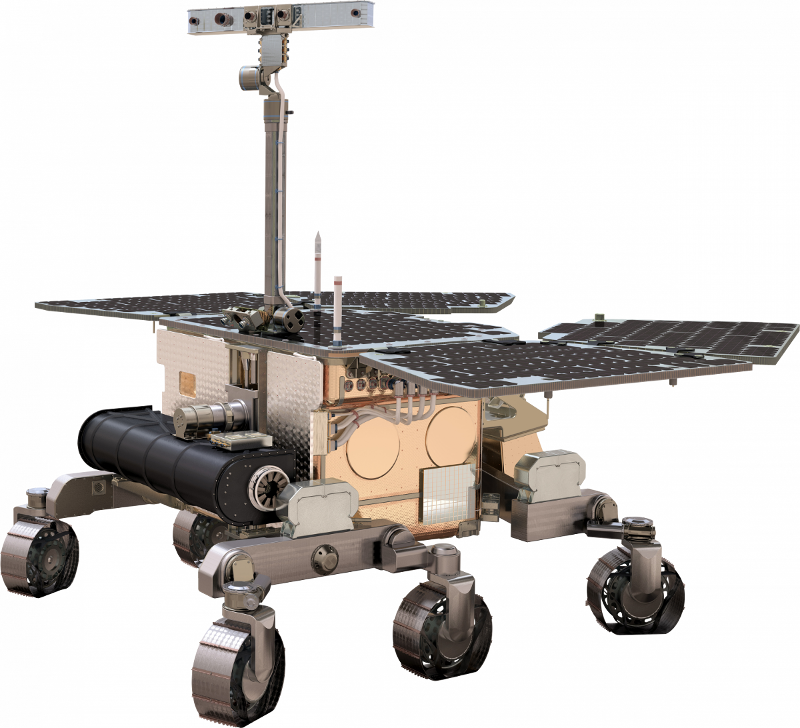
\includegraphics[height=\graphicsHeight]{sections/state-of-the-art/planned-missions/images/rover-exomars.png}
		\subcaption{Rosalind Franklin}
		\label{fig:sub:planned-mission-rover-exomars}
	\end{subfigure}
	\caption[Planned rover missions]
            {Planned rover missions. Mars 2020 is part of \ac{NASA}'s \ac{MEP}. Rosalind Franklin is part of the international ExoMars programme led by \ac{ESA} and Roscosmos}
	\label{fig:planned-mission-rovers}
\vspace{-2ex}
\end{figure}

\subsection{Mars 2020}
\label{sec:StateOfTheArt:PlannedMissions:Mars2020}

Mars 2020 is part of \ac{NASA}'s \ac{MEP}. Much of its design is based on heritage from the Curiosity mission. Its power system is identical to that of Curiosity in that it is equipped with a \ac{MMRTG} that will provide approximately \SI{110}{\watt} of electrical power at \ac{BOL}, declining by a few percent per year \citepower{Mars2020ElecticalPower}. Its two \ac{Li-ion} batteries are also identical to that of Curiosty and was previously elaborated on in \refSec{sec:StateOfTheArt:PastAndOngoingMissions:Rovers}.

\subsection{Rosalind Franklin}
\label{sec:StateOfTheArt:PlannedMissions:RosalindFranklin}

Rosalind Franklin is part of the international ExoMars programme led by \ac{ESA} and Roscosmos. Its \ac{SA} is designed to generate up to \SI{1200}{\watt\hour} of energy \citepower{SaftPressRelease}. The \ac{SA} power output requirements are:

\begin{itemize}
    \item \ac{BOL}: $P_{max} > \SI{261}{\watt}$ under \SI{471}{Wm^{-2}}, \SI{-26}{\celsius}, and one string fail.
    \item \ac{EOL}: $P_{max} > \SI{131}{\watt}$ under \SI{358}{Wm^{-2}}, \SI{-52}{\celsius}, \SI{34}{\percent} dust coverage, and one string fail plus losses.
\end{itemize}

Test results detailed in \citepower{Riva2019} have measured \ac{SA} performances of $P_{max} = \SI{277}{\watt}$ for \ac{BOL} and $P_{max} = \SI{133.4}{\watt}$ for \ac{EOL}. The rover's battery cells are arranged in a 8s3p configuration and have an operational temperature range of \SI{-40}{\celsius} to +\SI{85}{\celsius} \citepower{EDN}. The rover is equipped with \acp{RHU} in order to maintain its internal temperature above \SI{-40}{\celsius}. The \ac{Li-ion} battery cells are manufactured by Saft and have the following specifications:

\begin{itemize}
    \item Nominal voltage: 3.65 \si{\volt}.
    \item Voltage range: 2.5‒\SI{4.2}{\volt}.
    \item Nameplate capacity: \SI{5.6}{\ampere\hour}.
    \item Nameplate energy:
    \begin{itemize}
        \item \ac{BOL}: \SI{1140}{\watt\hour}  under +\SI{50}{\celsius}, \SI{50}{\percent}. \ac{SOC}.
        \item End of cruise: \SI{980}{\watt\hour} under +\SI{40}{\celsius}, \SI{50}{\percent} \ac{SOC}.
        \item \ac{EOL}: \SI{790}{\watt\hour} under \SI{-20}{\celsius}, \SI{40}{\percent}. \ac{DOD}.
    \end{itemize}
\end{itemize}

The battery characterstics taken from \citepower{Amos2017} are as follow:

\begin{itemize}
    \item Operating voltage: 21‒\SI{29.4}{\volt}.
    \item Mass: $<$ \SI{10.5}{\kilo\gram}.
    \item Charge current:
    \begin{itemize}
        \item T $>$ \SI{0}{\celsius}: up to \SI{3}{\ampere}.
        \item T $<$ \SI{0}{\celsius}: up to \SI{5.2}{\ampere}.
    \end{itemize}
    \item Discharge current:  up to \SI{15}{\ampere}.
\end{itemize}
